\documentclass[compress=true]{beamer}
\usepackage{caption}
%\usepackage{xeCJK}
%\setCJKmainfont{WenQuanYi Zen Hei}
\linespread{1.5}
\usetheme{Warsaw}
\title{Field Regions and Power Pattens of \\ Infinitesimal Dipole}
\author{\tiny{Yimian Dai,Wenbo Wang,Yu Qin,Haiyang Zhang}}
\institute{\url{http://dspandlinux.com}}
\begin{document}
% frame_01
\begin{frame}
\titlepage
\end{frame}
\begin{frame}
  \frametitle{Contents}
  \begin{figure}
    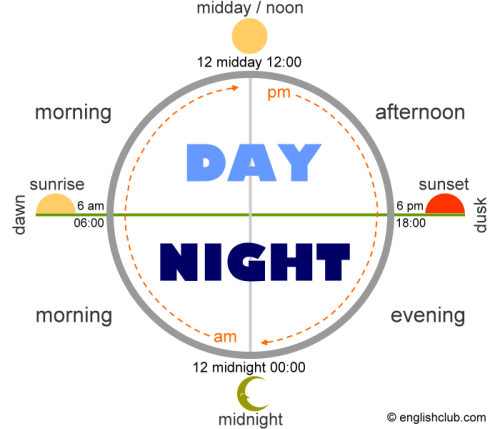
\includegraphics[height=0.8\textheight]{day-night.png}
%    \caption*{\tiny{kr=10000}}
  \end{figure}
\end{frame}
% frame_
\begin{frame}
  \frametitle{Antenna radiation zoning}
\begin{columns}
\begin{column}{0.7\textwidth}
{\it{\large{Infinitesimal Dipole(${l\ll \lambda}$)}}}
  \begin{itemize}
    \item Near-Field (kr$\ll$1) %Region
    \item Intermediate-Field (kr$>$1) %Region
    \item Far-Field (kr$\gg$1)
  \end{itemize}
\end{column}
\begin{column}{0.3\textwidth}
  \begin{figure}
    
\includegraphics[height=0.2\textheight]{sunny_happy_day.png}
%    \caption*{\tiny{kr=10000}}
  \end{figure}
{\huge \em{Why ?\\
How ?\\
What ?\\}}
\end{column}
\end{columns}
\end{frame}
% frame_
\begin{frame}
  \frametitle{Outline}
  \begin{block}{\bf E}
    $$E_r = \eta\frac{I_0l\cos{\theta}}{2\pi r^2}[1+\frac{1}{jkr}]e^{-jkr}$$
    $$E_{\theta} = j\eta\frac{kI_0l\sin{\theta}}{4\pi r}[1+\frac{1}{jkr}-\frac{1}{(kr)^2}]e^{-jkr}$$
    $$E_{\phi}=0$$
  \end{block}
  \begin{block}{\bf H}
    $$H_r=H_{\theta}=0$$
    $$H_{\phi}=j\frac{kI_0l\sin{\theta}}{4\pi r}[1+\frac{1}{jkr}]e^{-jkr}$$
  \end{block}
\end{frame}
\begin{frame}
	\frametitle{Outline}
\begin{block}{Poynting vector}
	$$
		\begin{array}{ll}
			{\bf W} & =\frac{1}{2}({\bf E}\times{\bf
			H}^*)=\frac{1}{2}(\hat{a}_rE_r+\hat{a}_{\theta}E_{\theta})\times(\hat{a}_{\phi}H_{\phi}^*)\\
		{}	&
			=\frac{1}{2}(\hat{a}_rE_{\theta}H_{\phi}^* - \hat{a}_{\phi}E_rH_{\phi}^*)
		\end{array}
	$$
\end{block}
\begin{block}{Power}
    $$
        \begin{array}{ll}
          P & =\frac{1}{2}\iint\limits_s {\bf E}\times{\bf H}^*{\cdot}d{\bf s}=\eta(\frac{\pi}{3})|\frac{I_0l}{\lambda}|^2[1-j\frac{1}{(kr)^3}]\\
          {}  & =P_{rad}+j2\omega({\tilde{W}_m-\tilde{W}_e})
          \end{array}
    $$
\end{block}
\end{frame}

\begin{frame}
  \frametitle{Outline}
 \begin{figure}
    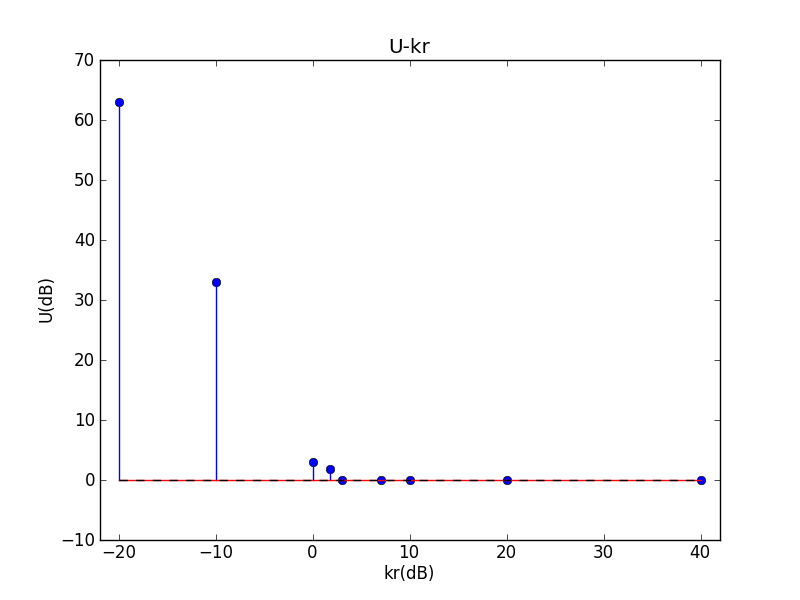
\includegraphics[height=0.8\textheight]{ratio.png}
  \end{figure}
\end{frame}

%% Near
% frame_
\begin{frame}
  \frametitle{Near-Field Region}
\begin{block}{~}
  \begin{equation}
    \left.
      \begin{array}{l}
        E_r \simeq -j{\eta}\frac{I_0le^{-jkr}}{2\pi kr^3}\cos{\theta}\\
        E_{\theta} \simeq -j{\eta}\frac{I_0le^{-jkr}}{1\pi kr^3}\sin{\theta}\\
        E_{\phi}=H_r=H_{\theta}=0\\
        H_{\phi}\simeq \frac{I_0le^{-jkr}}{4\pi r^2}\sin{\theta}
      \end{array}
    \right\}~~~~ kr\ll 1
  \end{equation}
\end{block}
\begin{center}
if~~$f=10GHz,kr=0.1$,then\\
$k=\frac{2\pi}{\lambda}=\frac{2\pi f}{c}\simeq 209.4$\\
so~$r=0.000477 m$
\end{center}
\end{frame}
% frame_
\begin{frame}
  \frametitle{Patten of Near-Field Region}
%  \framesubtitle{kr=0.01}
  \begin{figure}
    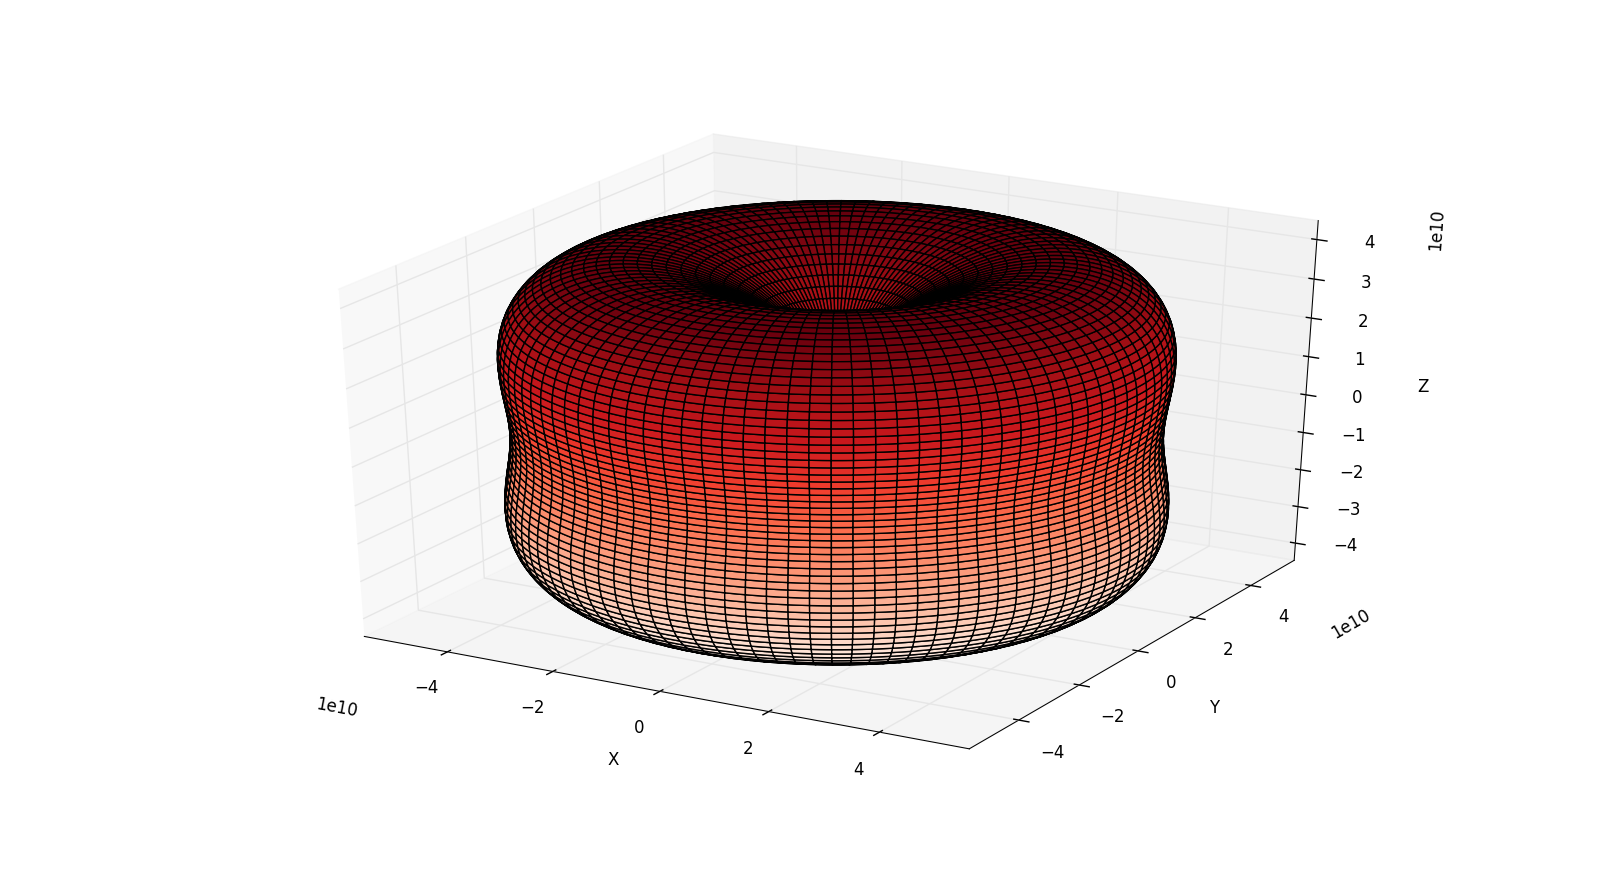
\includegraphics[height=0.68\textheight]{near_kr_0_01_1.png}
    \caption*{\tiny{kr=0.01}}
  \end{figure}
\end{frame}
% frame_
\begin{frame}
  \frametitle{Patten of Near-Field Region}
%\begin{center}{\tiny kr=0.1}\end{center}
  \begin{figure}
    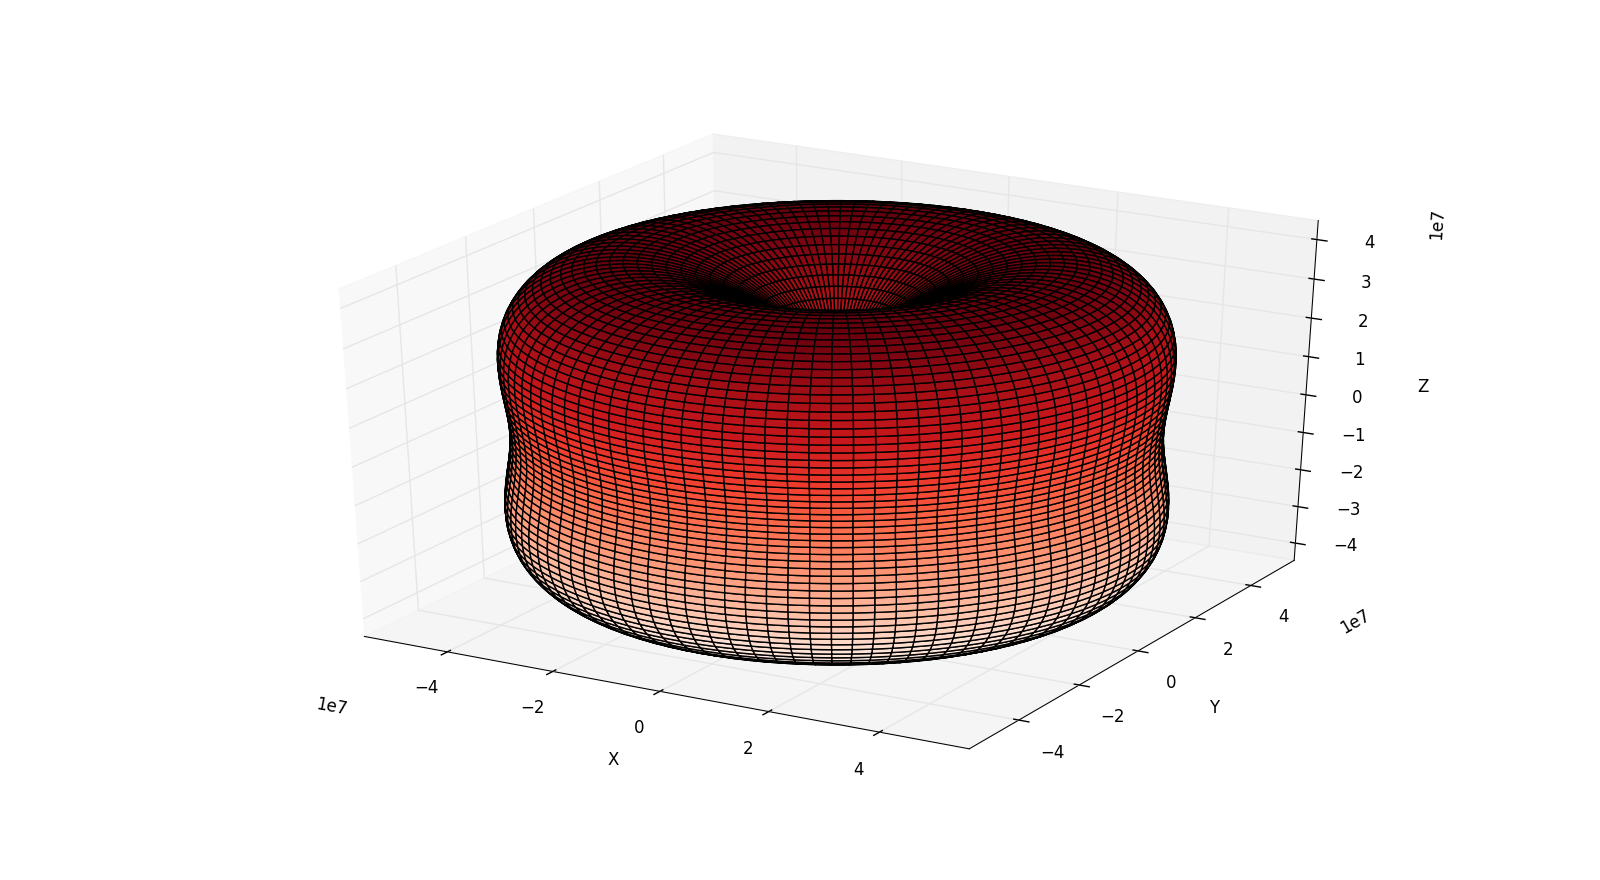
\includegraphics[height=0.68\textheight]{near_kr_0_1_1.png}
    \caption*{\tiny{kr=0.1}}
  \end{figure}
\end{frame}
% frame_
\begin{frame}
  \frametitle{Patten of Near-Field Region}
  \begin{figure}
    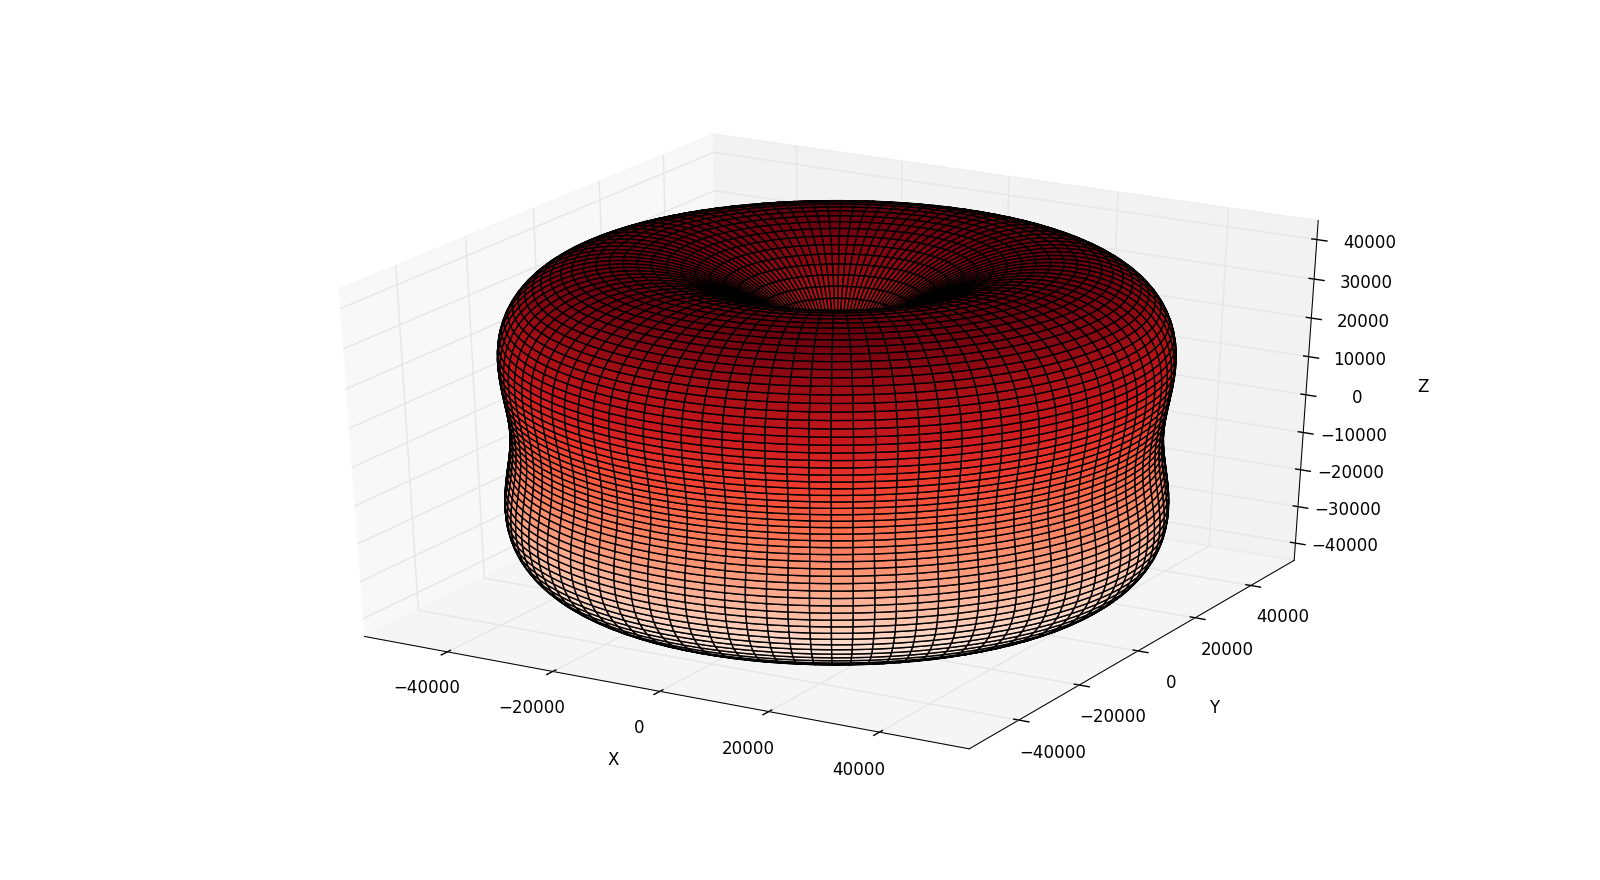
\includegraphics[height=0.68\textheight]{near_kr_1_1.png}
    \caption*{\tiny{kr=1}}
  \end{figure}
\end{frame}


%% Inter
% frame_
\begin{frame}
  \frametitle{Patten of Intermediate-Field Region}
  \begin{block}{~}
  \begin{equation}
    \left.
      \begin{array}{l}
        E_r \simeq {\eta}\frac{I_0le^{-jkr}}{1\pi r^1}\cos{\theta}\\
        E_{\theta} \simeq j{\eta}\frac{kI_0le^{-jkr}}{4\pi r}\sin{\theta}\\
        E_{\phi}=H_r=H_{\theta}=0\\
        H_{\phi}\simeq j\frac{kI_0le^{-jkr}}{4\pi r}\sin{\theta}
      \end{array}
    \right\} kr>1 
  \end{equation}
\end{block}
\end{frame}
% frame_
\begin{frame}
  \frametitle{Patten of Intermediate-Field Region}
  \begin{figure}
    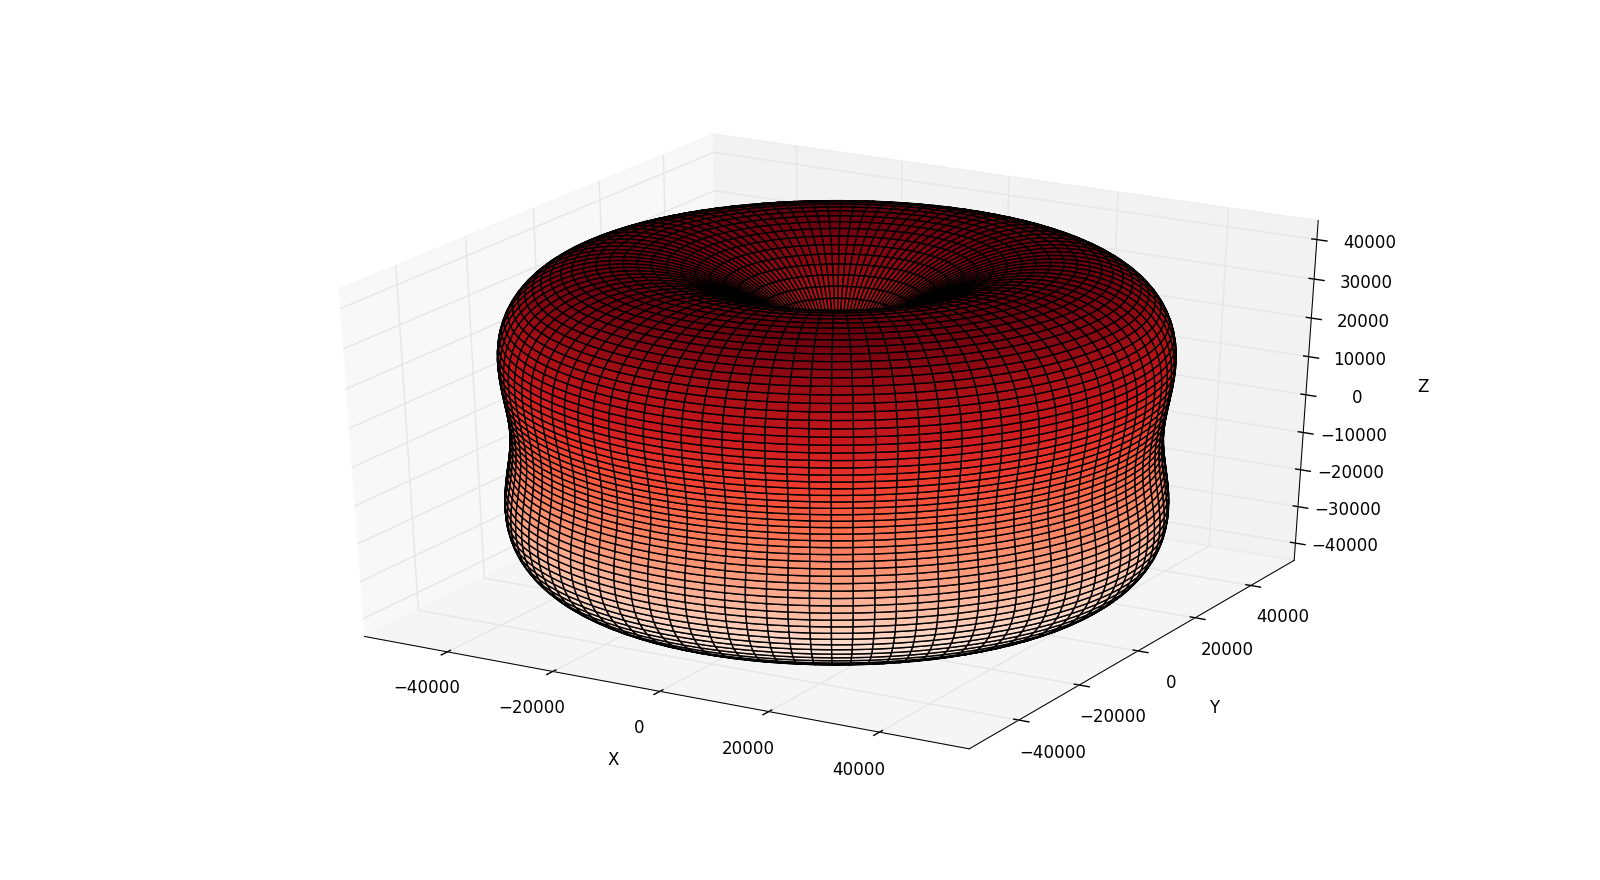
\includegraphics[height=0.68\textheight]{inter_kr_1_1.png}
    \caption*{\tiny{kr=1}}
  \end{figure}
\end{frame}
% frame_
\begin{frame}
  \frametitle{Patten of Intermediate-Field Region}
  \begin{figure}
    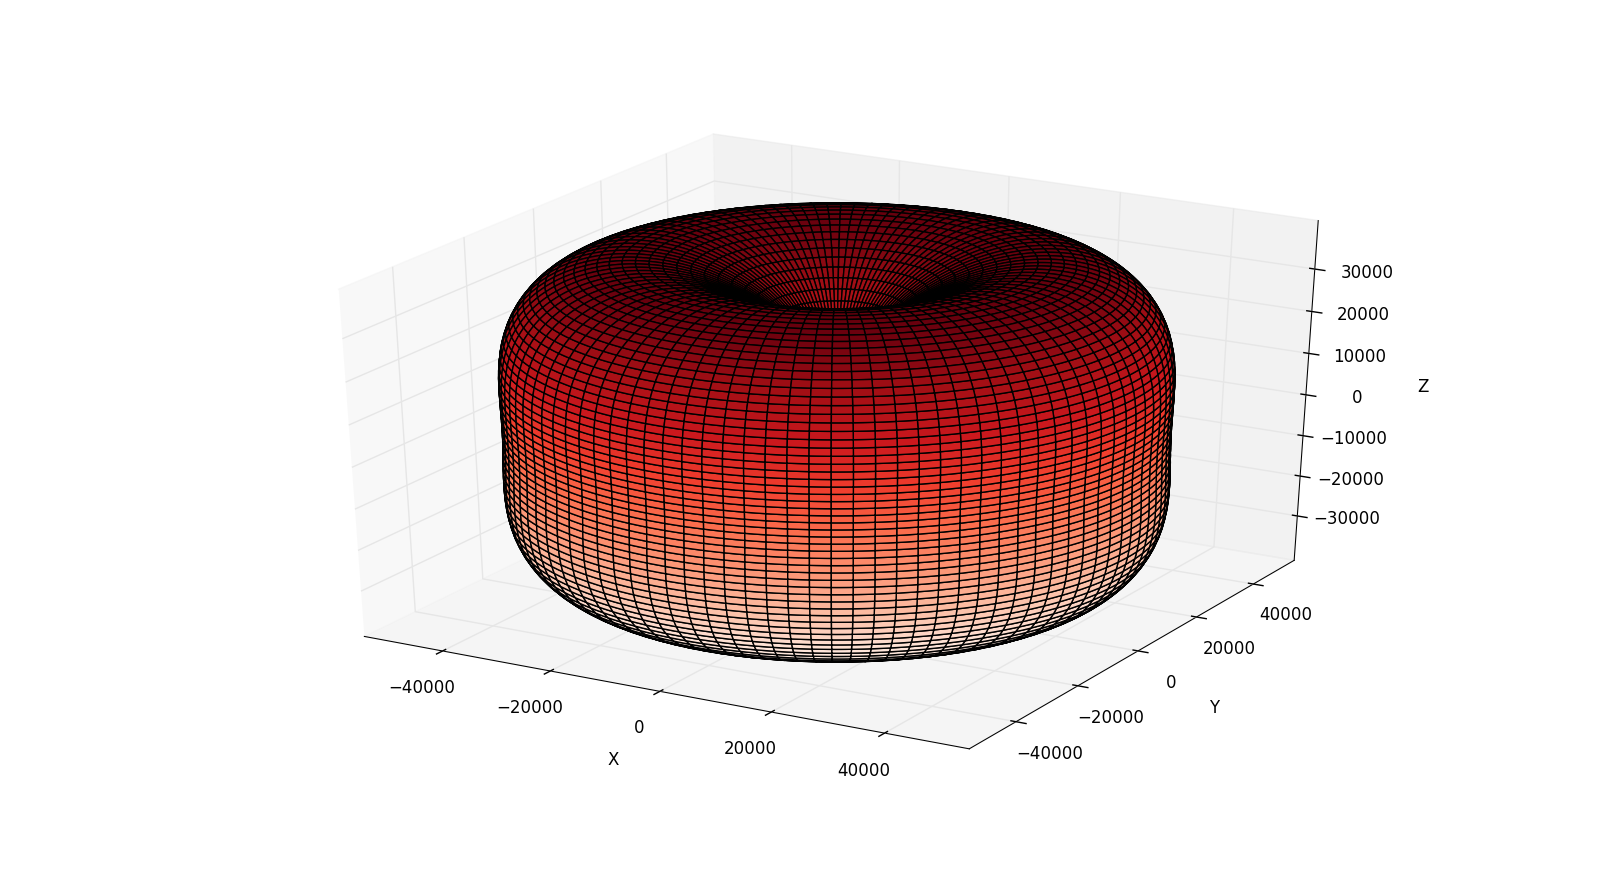
\includegraphics[height=0.68\textheight]{inter_kr_1_1_1.png}
    \caption*{\tiny{kr=1.1}}
  \end{figure}
\end{frame}
% frame_
\begin{frame}
  \frametitle{Patten of Intermediate-Field Region}
  \begin{figure}
    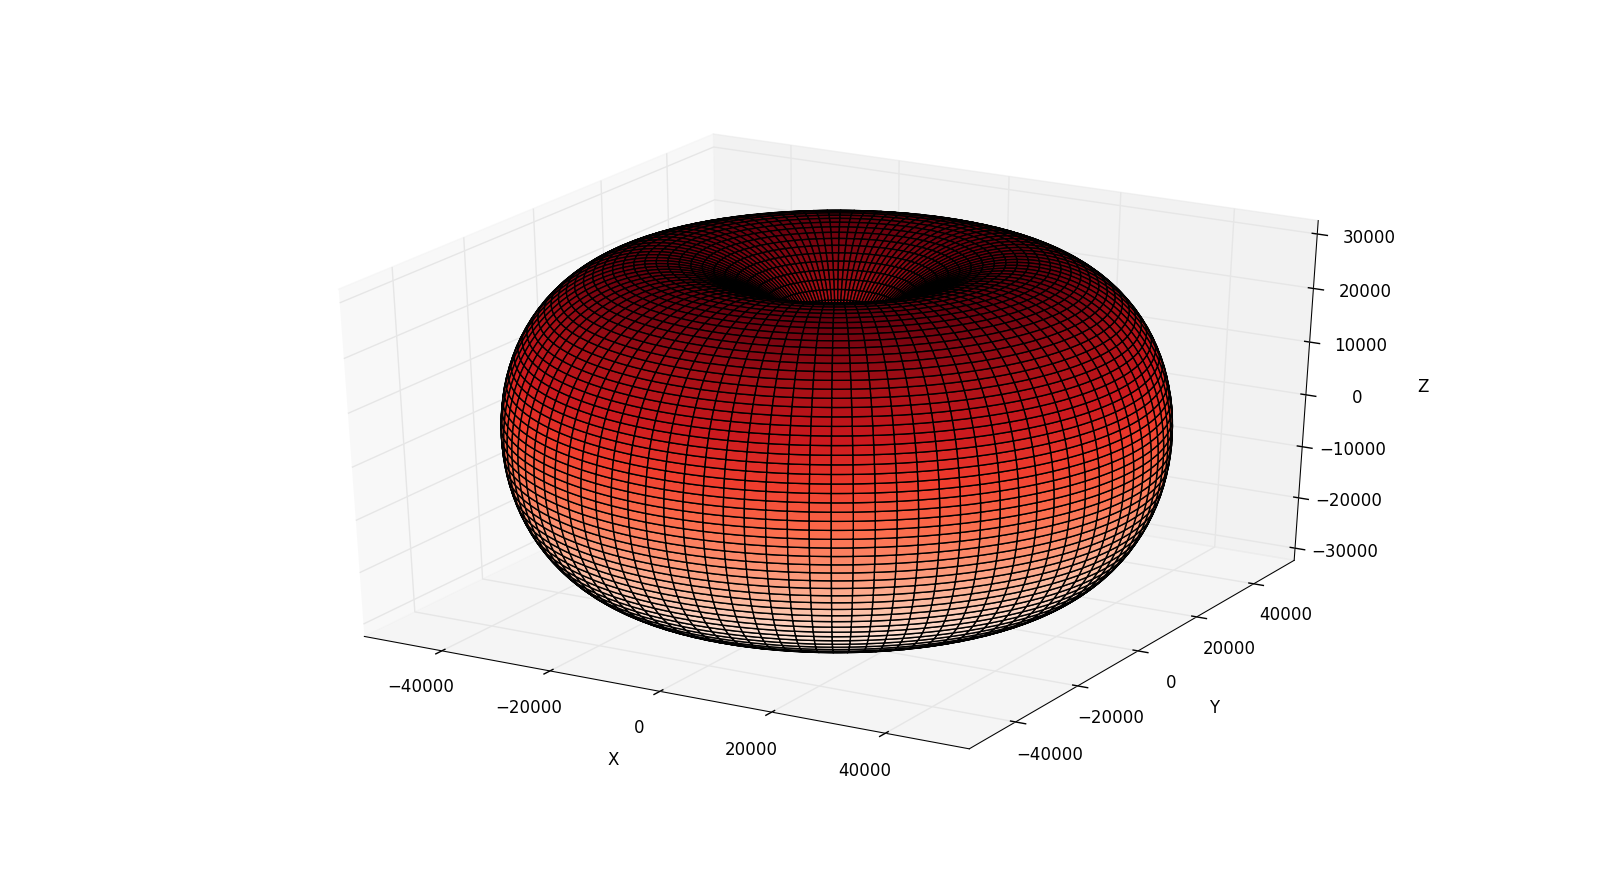
\includegraphics[height=0.68\textheight]{inter_kr_1_5_1.png}
    \caption*{\tiny{kr=1.5}}
  \end{figure}
\end{frame}
% frame_
\begin{frame}
  \frametitle{Patten of Intermediate-Field Region}
  \begin{figure}
    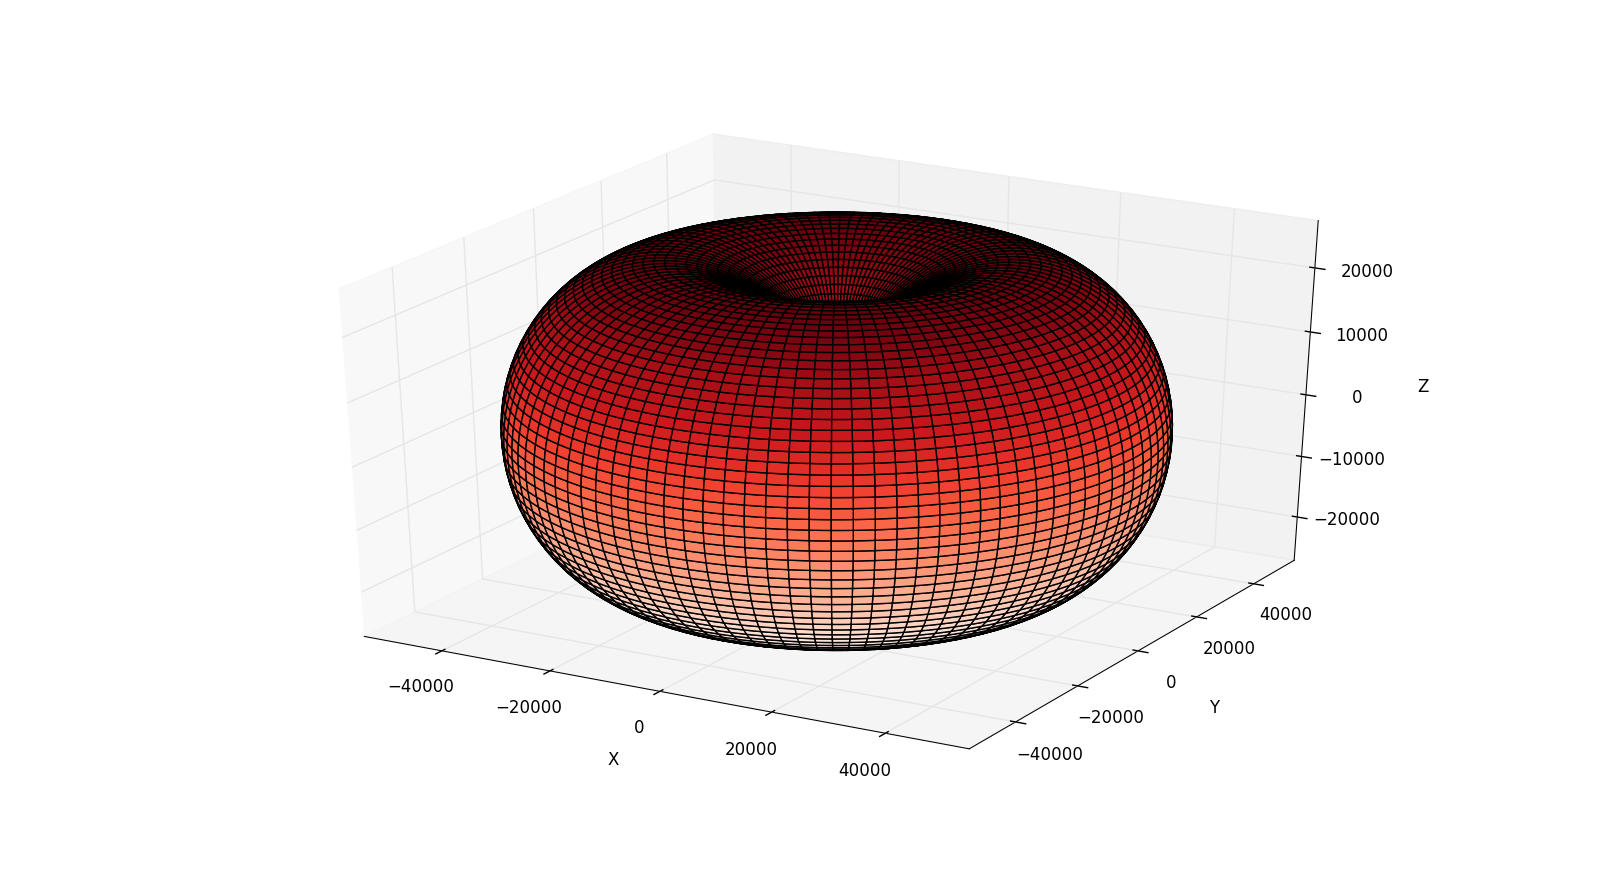
\includegraphics[height=0.68\textheight]{inter_kr_2_1.png}
    \caption*{\tiny{kr=2}}
  \end{figure}
\end{frame}
% frame_
\begin{frame}
  \frametitle{Patten of Intermediate-Field Region}
  \begin{figure}
    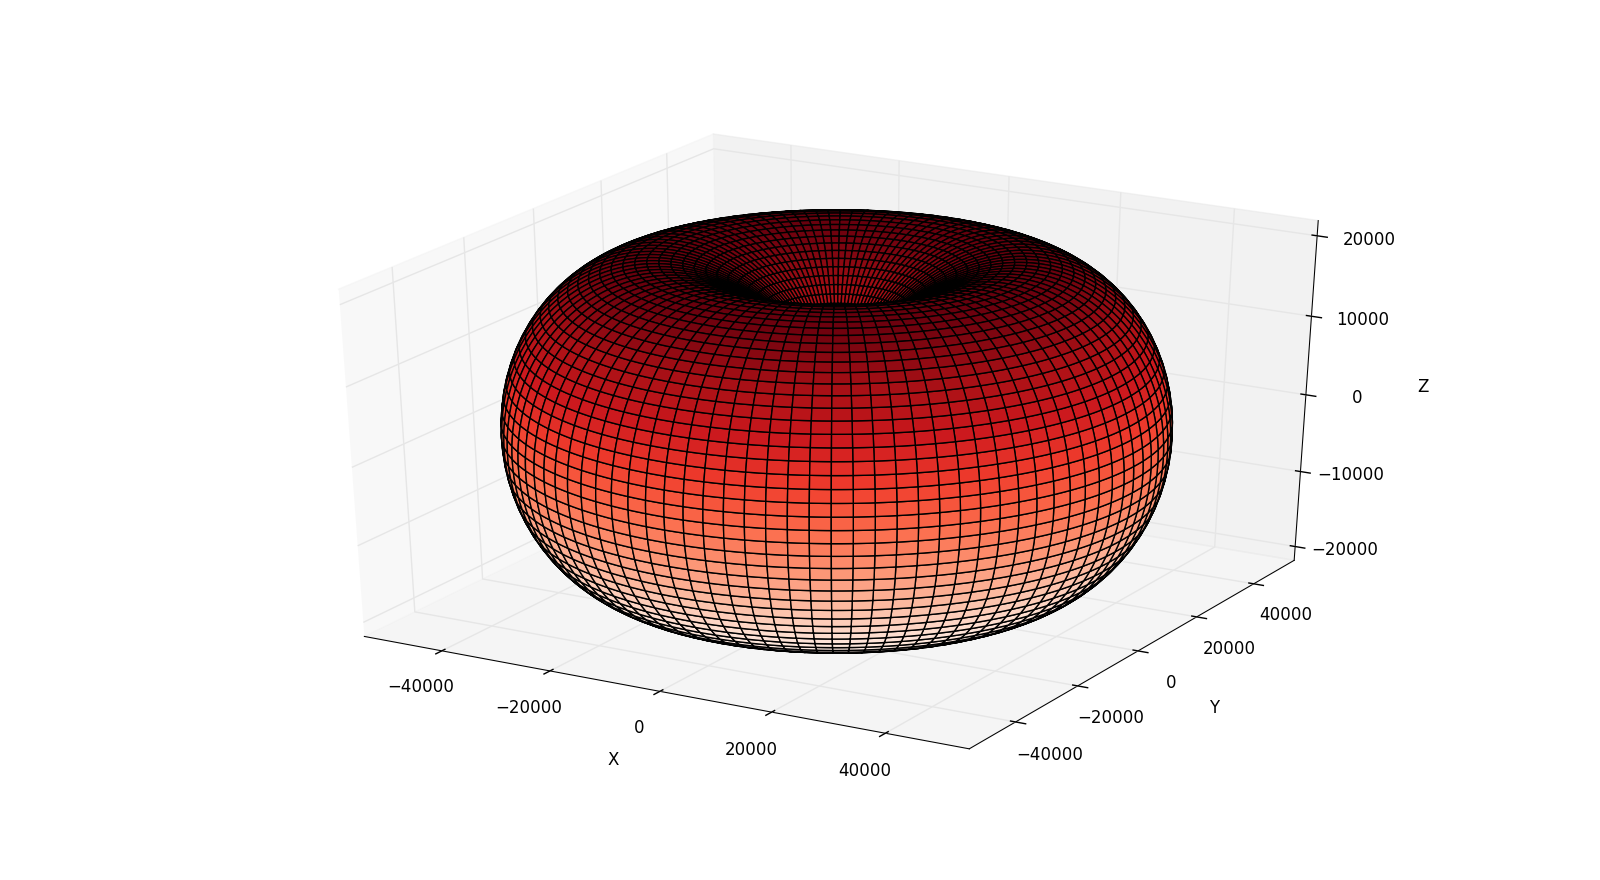
\includegraphics[height=0.68\textheight]{inter_kr_5_1.png}
    \caption*{\tiny{kr=5}}
  \end{figure}
\end{frame}



%% far
% frame_
\begin{frame}
  \frametitle{Far-Field Region}
  \begin{block}{~}
  \begin{equation}
    \left.
      \begin{array}{l}
        E_{\theta} \simeq j{\eta}k\frac{I_0le^{-jkr}}{4\pi r}\sin{\theta}\\
        E_r=E_{\phi}=H_r=H_{\theta}=0\\
        H_{\phi}\simeq j\frac{kI_0le^{-jkr}}{4\pi r}\sin{\theta}
      \end{array}
    \right\} kr\gg 1
  \end{equation}
  \end{block}
\end{frame}
% frame_
\begin{frame}
  \frametitle{Patten of Far-Field Region}
%  \framesubtitle{kr=0.01}
  \begin{figure}
    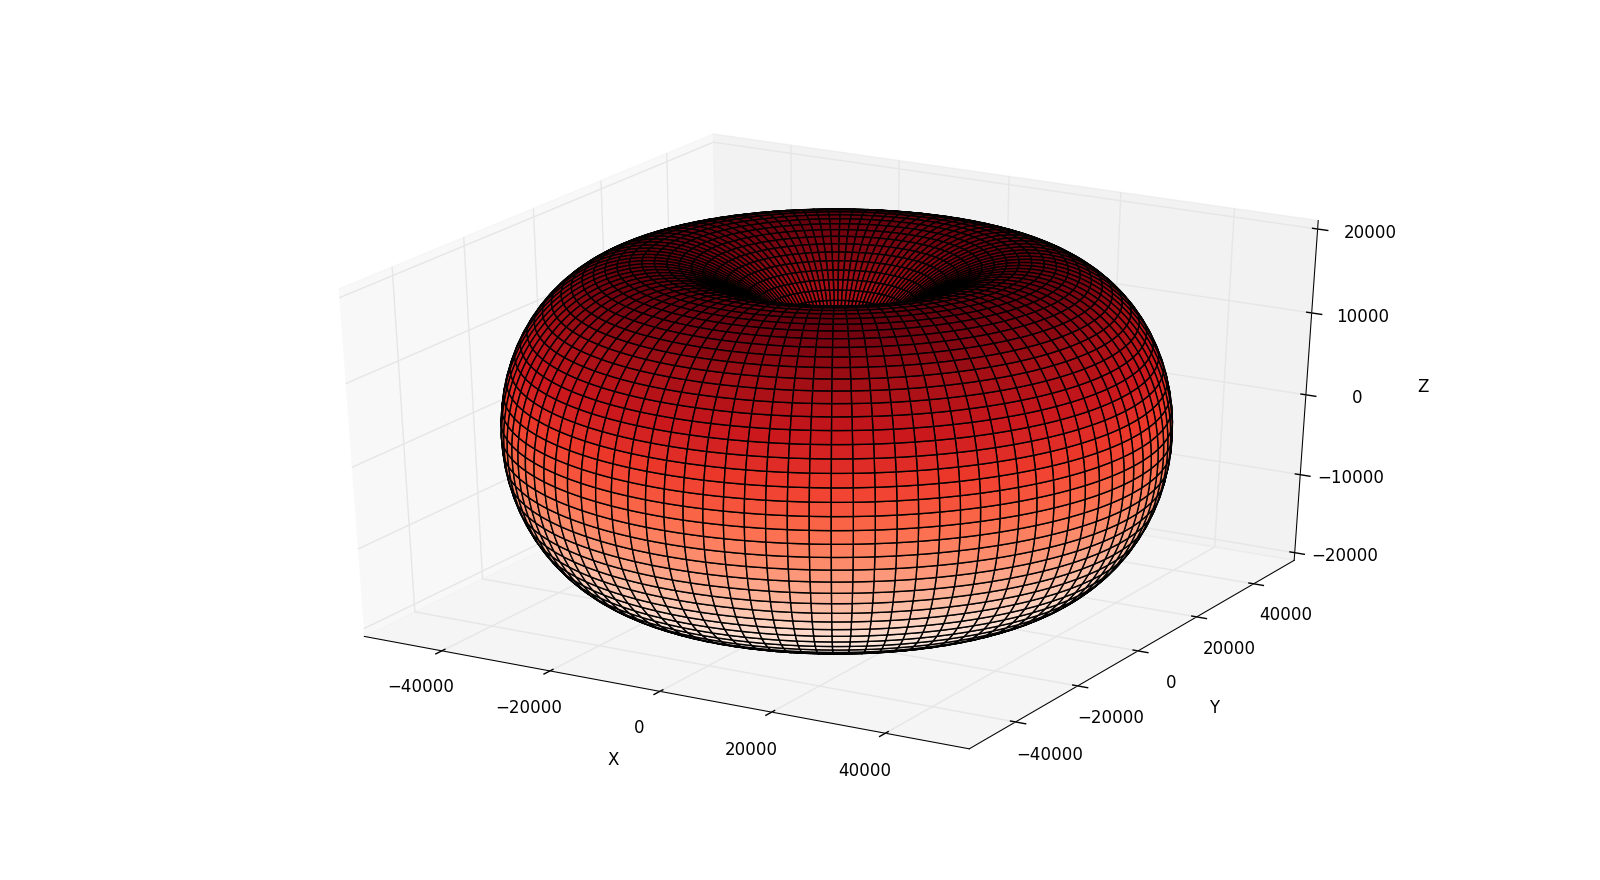
\includegraphics[height=0.68\textheight]{far_kr_10_1.png}
    \caption*{\tiny{kr=10}}
  \end{figure}
\end{frame}
\begin{frame}
  \frametitle{Patten of Far-Field Region}
%  \framesubtitle{kr=0.01}
  \begin{figure}
    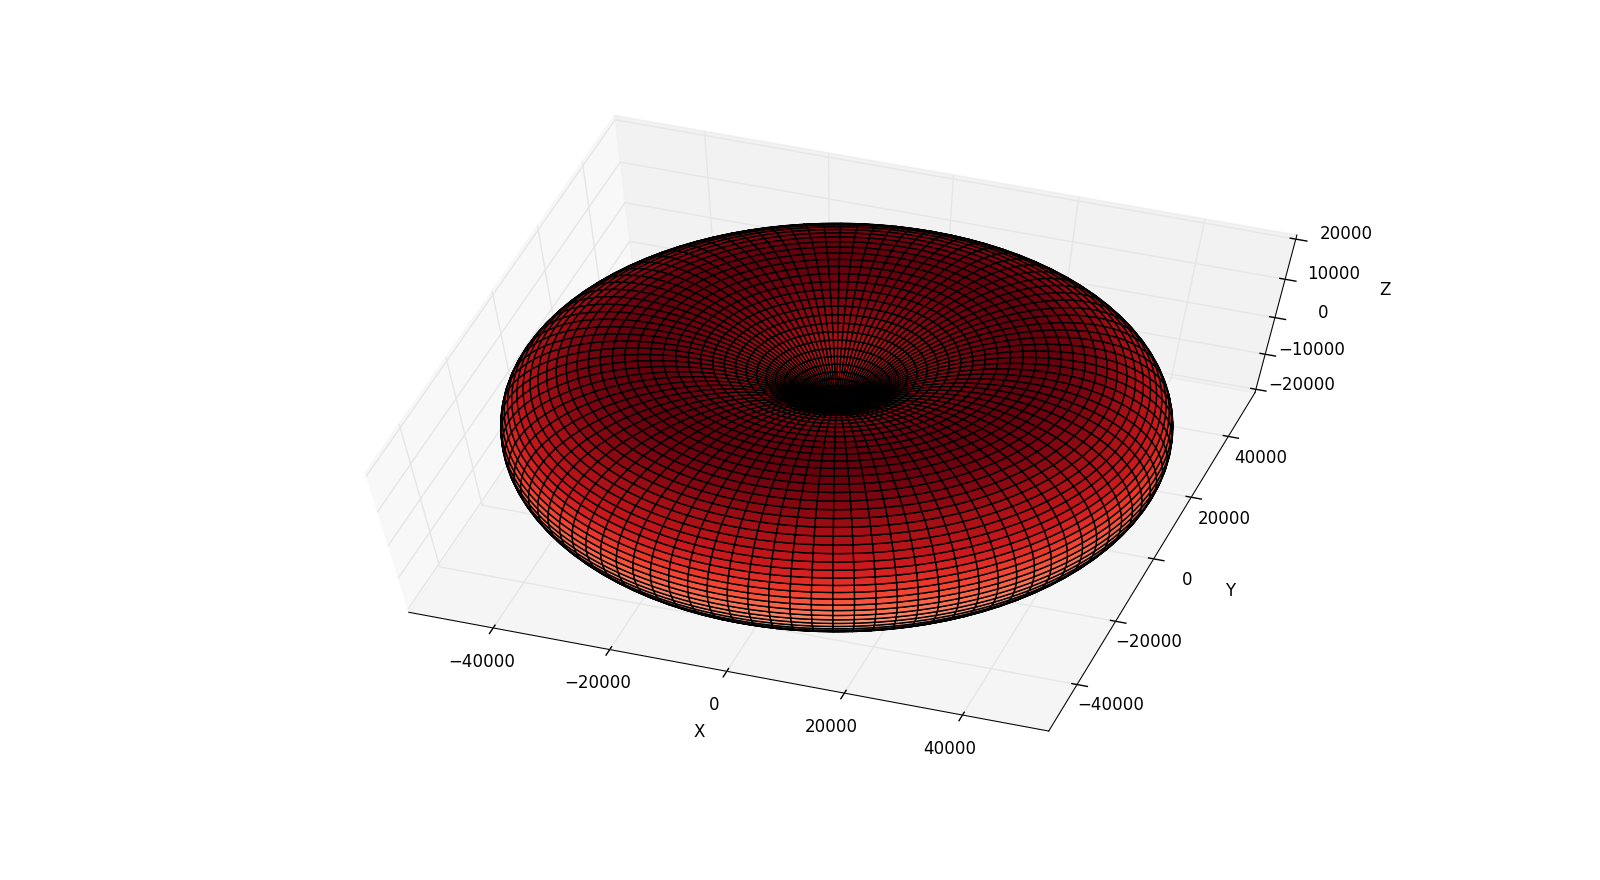
\includegraphics[height=0.68\textheight]{far_kr_10_2.png}
    \caption*{\tiny{kr=10}}
  \end{figure}
\end{frame}
\begin{frame}
  \frametitle{Patten of Far-Field Region}
%  \framesubtitle{kr=0.01}
  \begin{figure}
    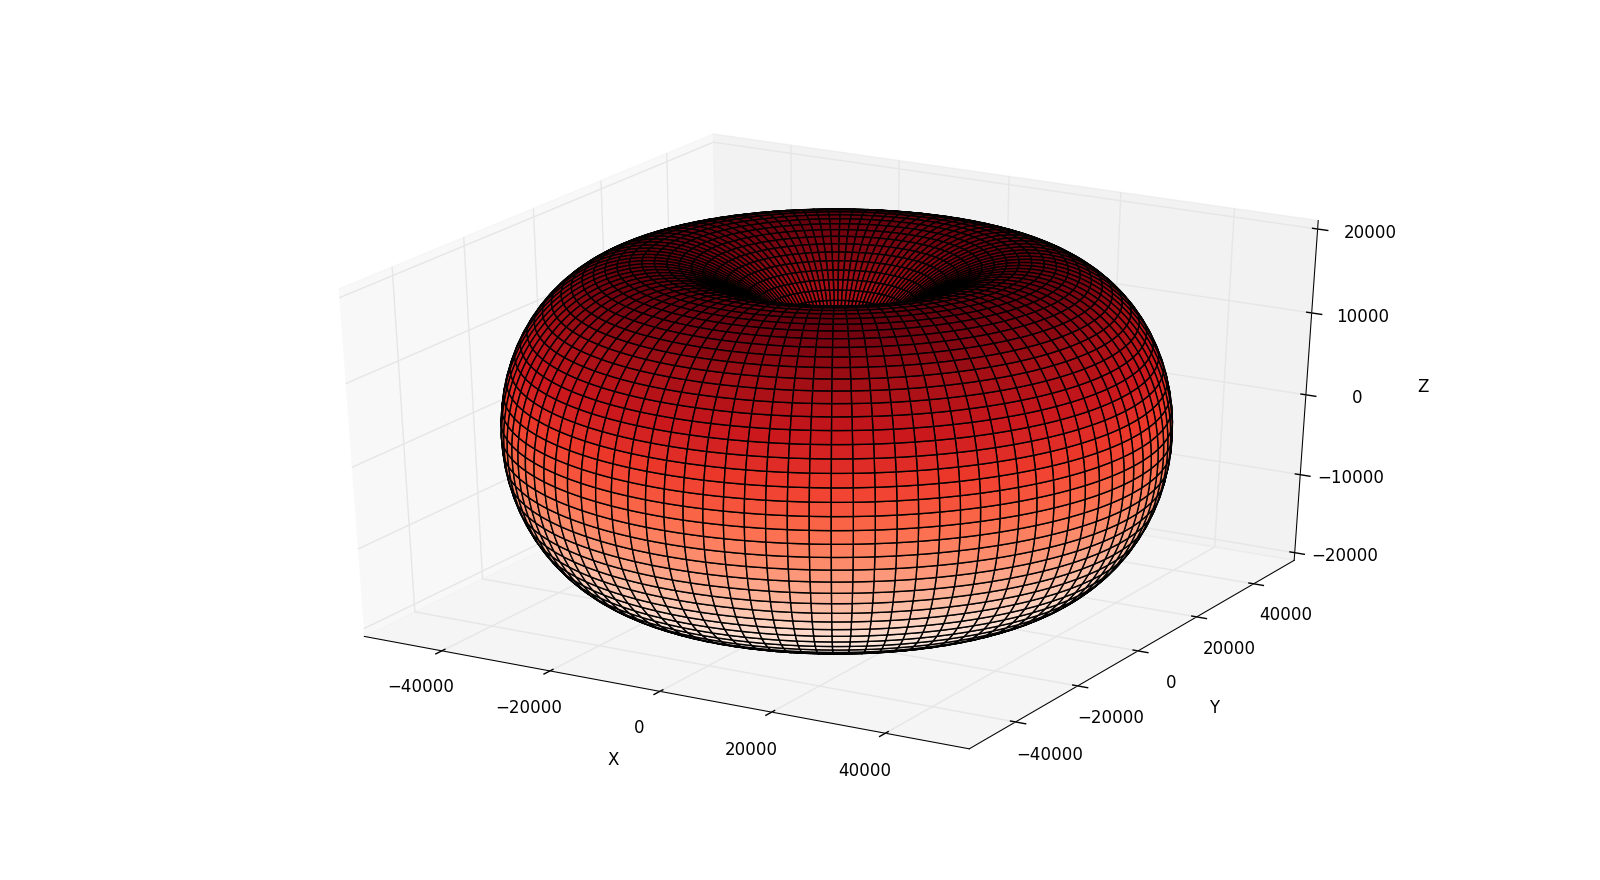
\includegraphics[height=0.68\textheight]{far_kr_100_1.png}
    \caption*{\tiny{kr=100}}
  \end{figure}
\end{frame}
\begin{frame}
  \frametitle{Patten of Far-Field Region}
%  \framesubtitle{kr=0.01}
  \begin{figure}
    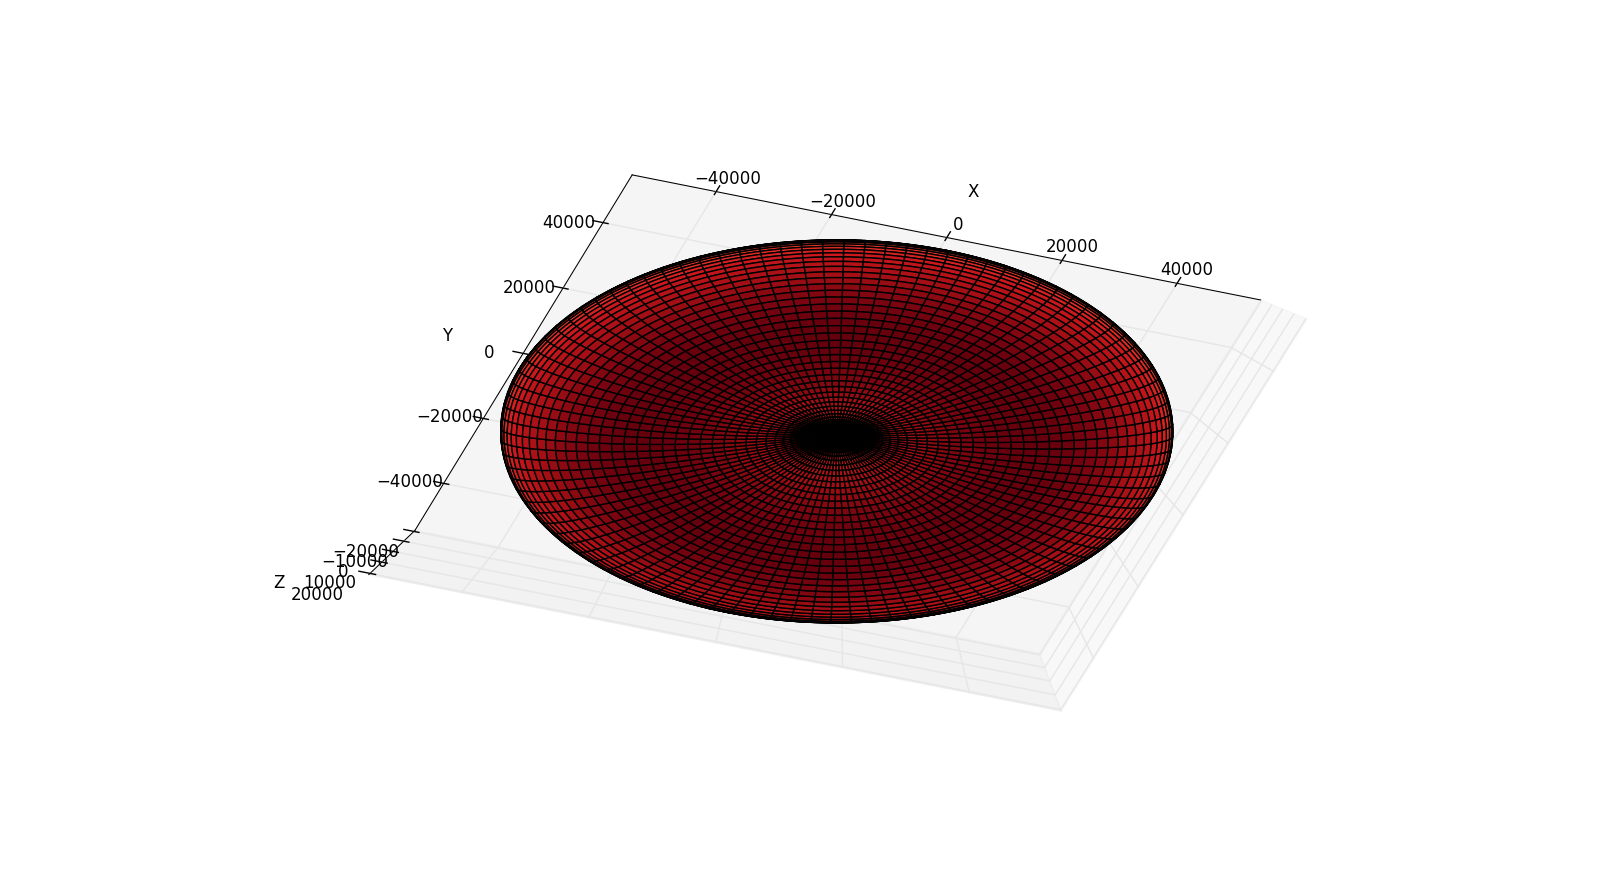
\includegraphics[height=0.68\textheight]{far_kr_100_2.png}
    \caption*{\tiny{kr=100}}
  \end{figure}
\end{frame}
% frame_
\begin{frame}
  \frametitle{Patten of Far-Field Region}
  \begin{figure}
    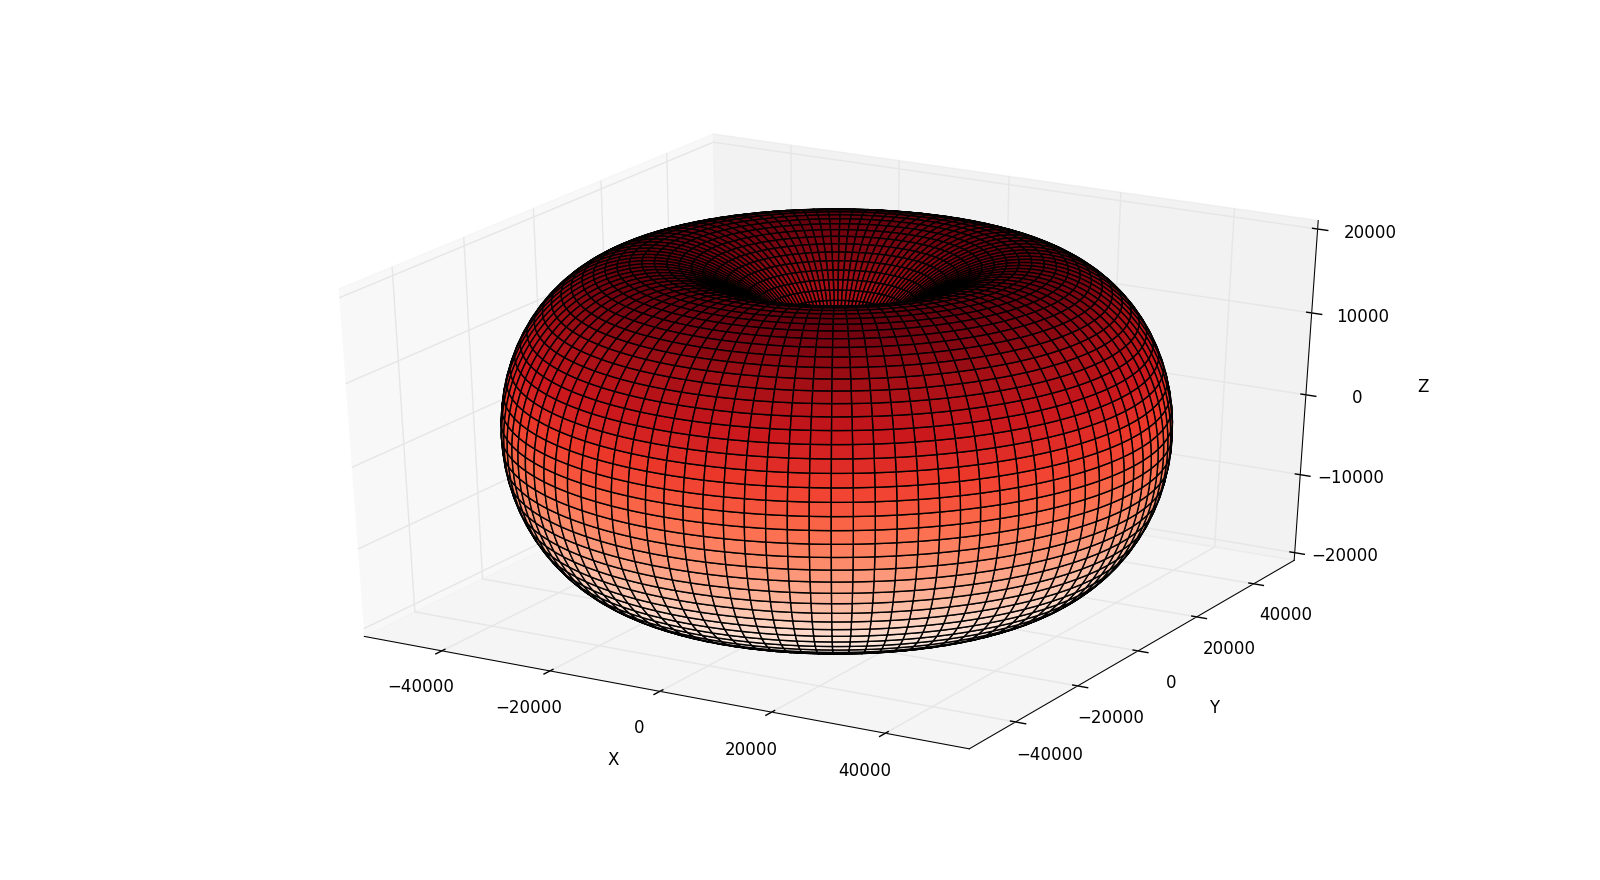
\includegraphics[height=0.68\textheight]{far_kr_10000_1.png}
    \caption*{\tiny{kr=10000}}
  \end{figure}
\end{frame}



\begin{frame}
  \frametitle{\it flapdoodle}
  \begin{figure}
    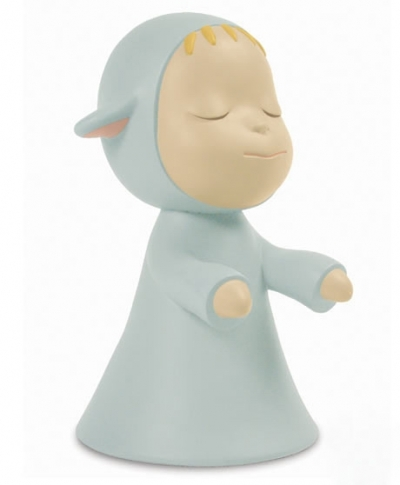
\includegraphics[height=0.68\textheight]{mengyou.jpg}
%    \caption*{\tiny{kr=10000}}
  \end{figure}
\end{frame}

\begin{frame}
  \frametitle{Sidelobe}
\begin{center}$Interference \Rightarrow Sidelobe$\end{center}
\begin{columns}
  \begin{column}{0.5\textwidth}
  \begin{figure}
    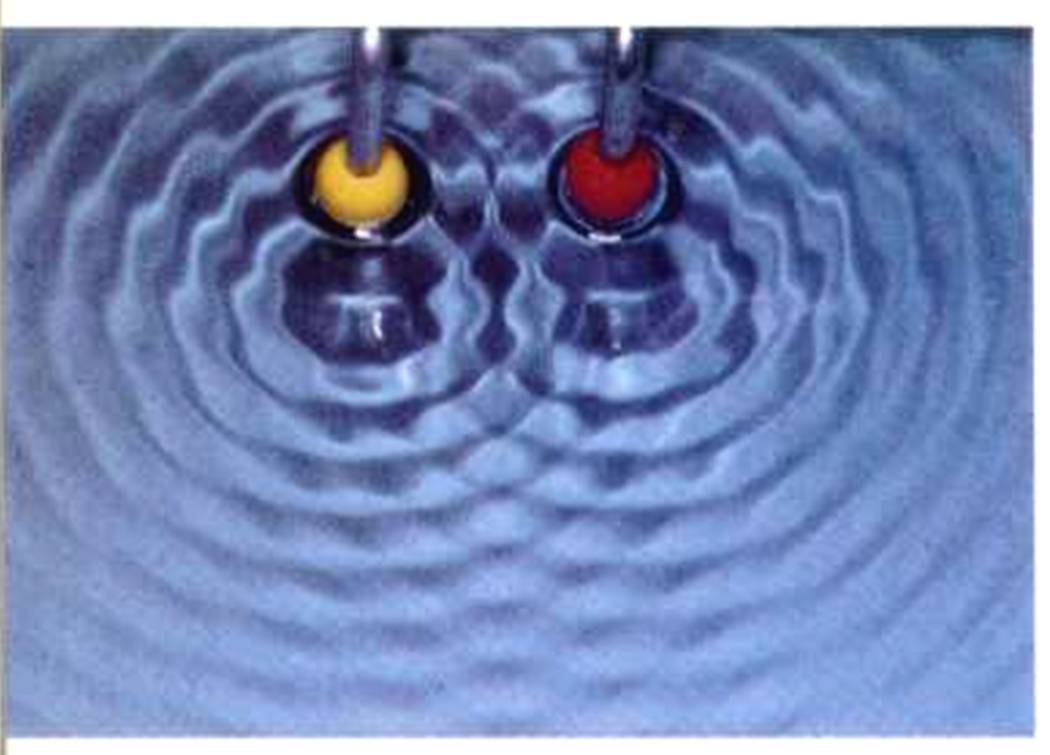
\includegraphics[height=0.4\textheight]{water.jpg}
%    \caption*{\tiny{kr=10000}}
  \end{figure}
\end{column}
\begin{column}{0.5\textwidth}
  \begin{figure}
    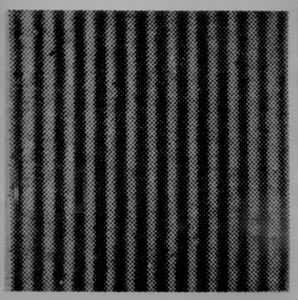
\includegraphics[height=0.5\textheight]{guang.jpg}
%    \caption*{\tiny{kr=10000}}
  \end{figure}
\end{column}
\end{columns}
\end{frame}


\begin{frame}
  \frametitle{Array Factor}
   \begin{figure}
    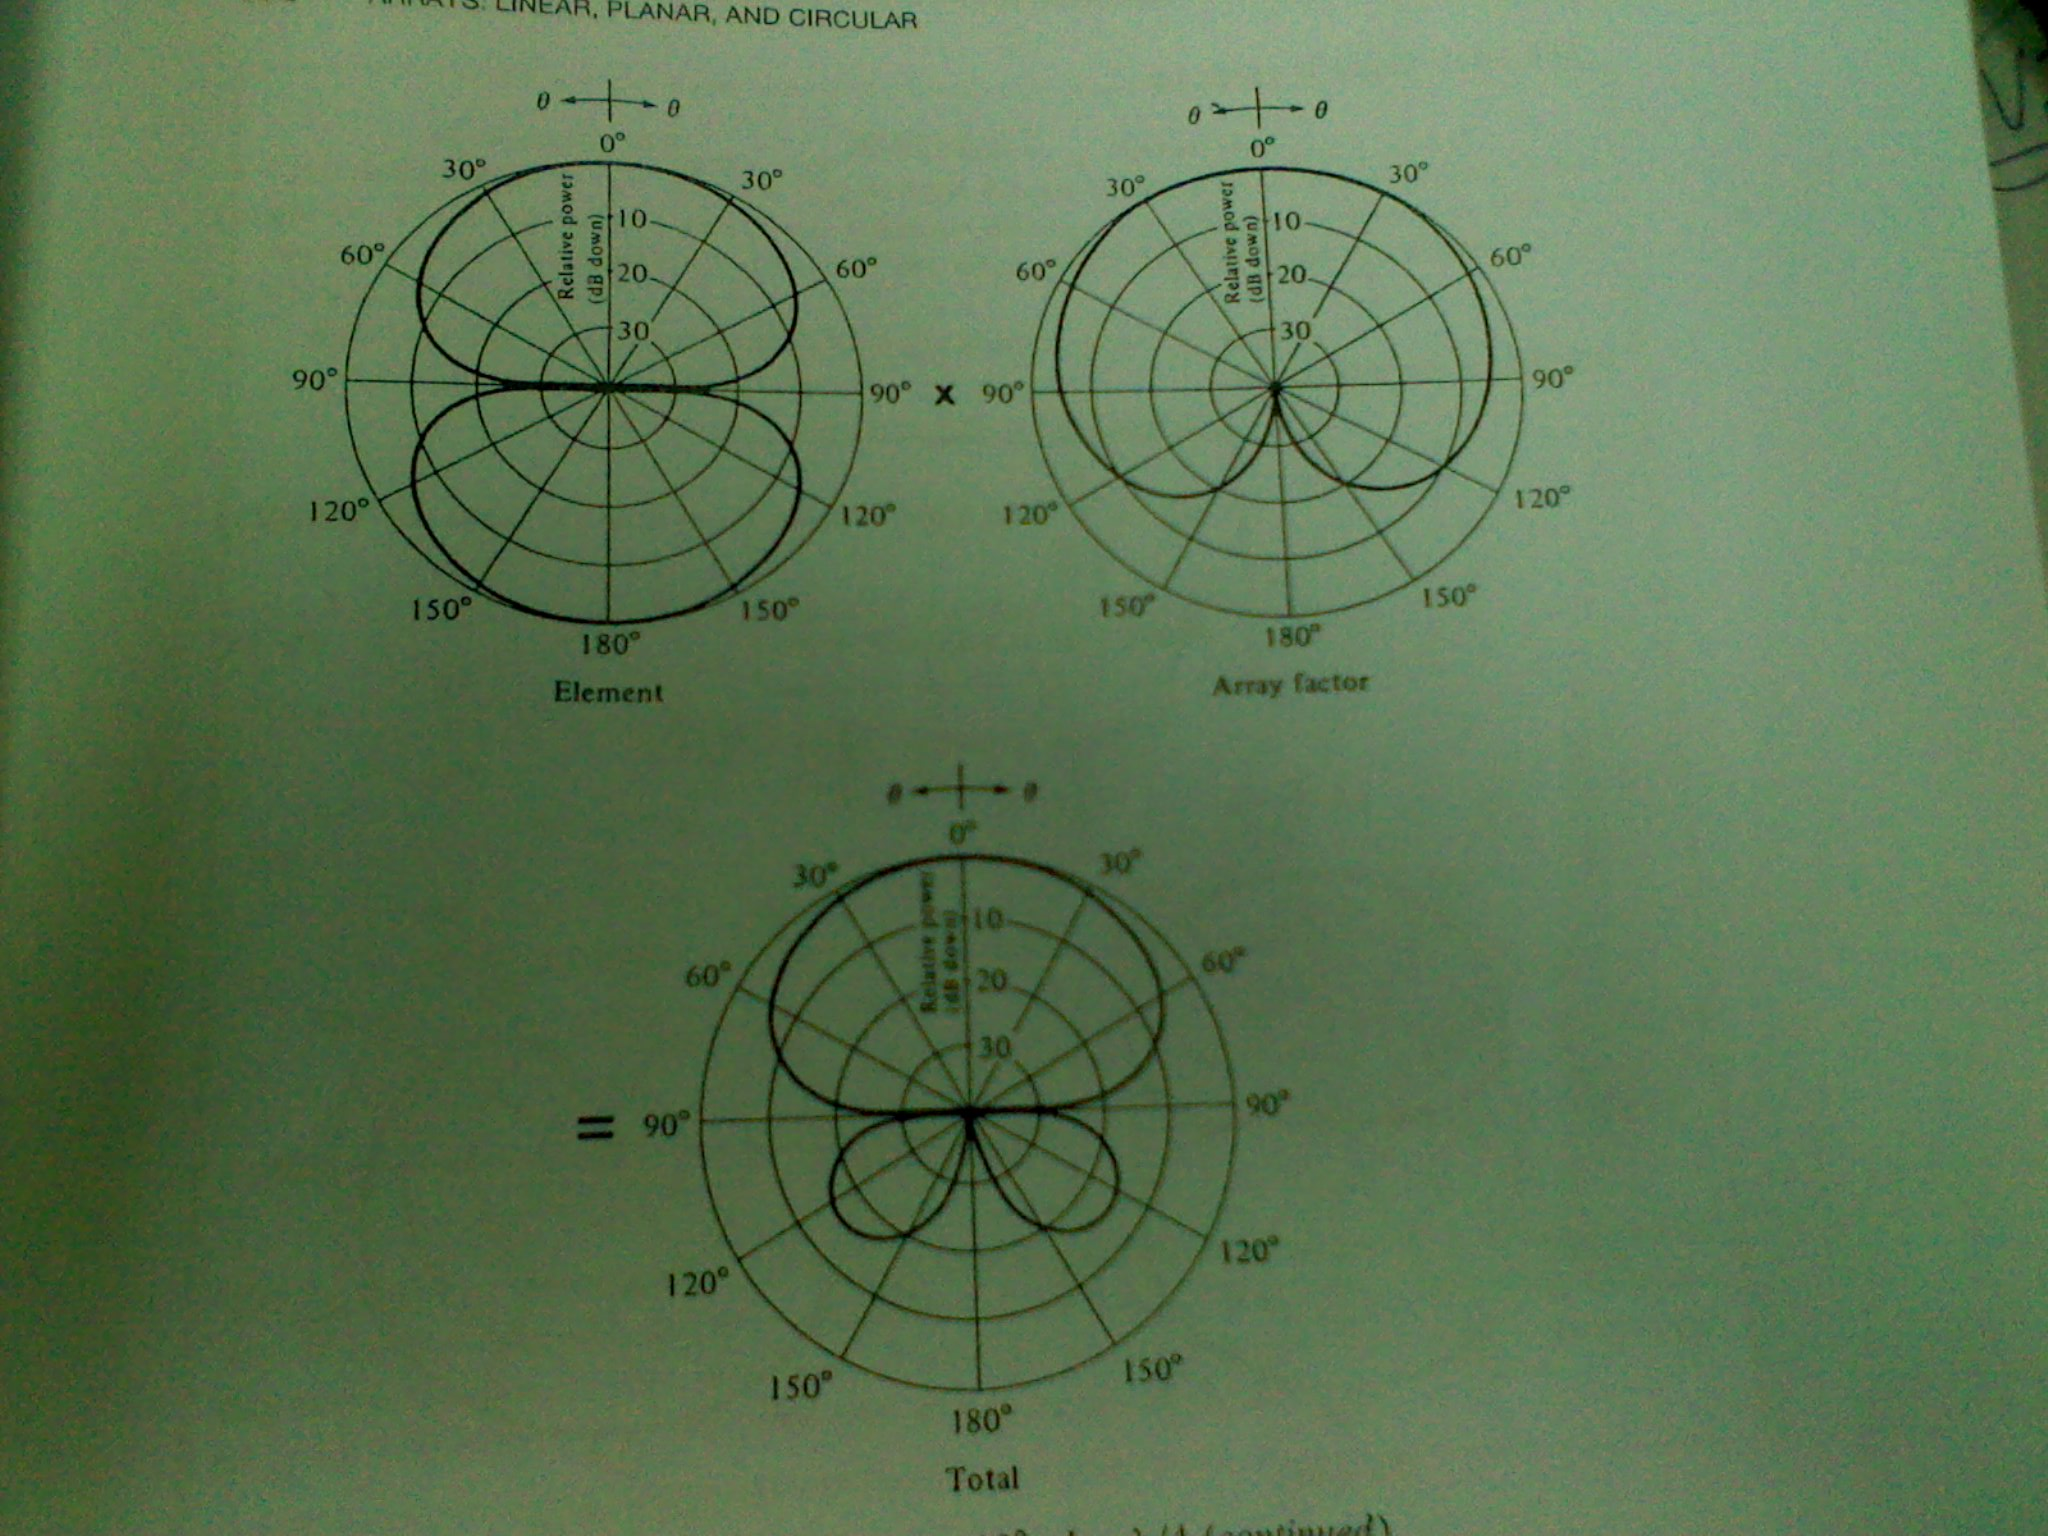
\includegraphics[height=0.8\textheight]{af.jpg}
%    \caption*{\tiny{kr=10000}}
  \end{figure}

\end{frame}
 
\begin{frame}
\frametitle{Fourier transform}
\begin{columns}
\begin{column}{0.7\textwidth}
\begin{block}{\bf A}
$$
{\bf A}(x,y,z)=\frac{\mu}{4\pi}\int_C{\bf I}_e(x',y',z')\frac{e^{-jkR}}{R}dl'$$
$${\tiny{R\simeq r-z'\cos{\theta}}}$$
\end{block}
\end{column}
\begin{column}{0.3\textwidth}
  \begin{figure}
    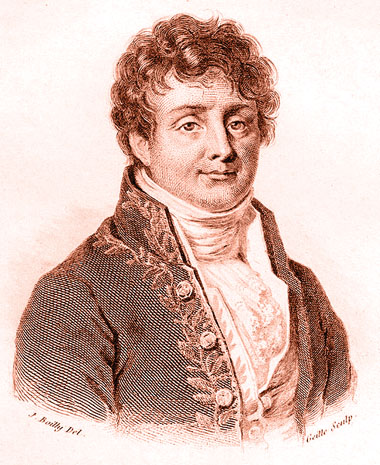
\includegraphics[height=0.3\textheight]{Fourier.jpg}
  \end{figure}
\end{column}
\end{columns}
\begin{block}{$E_{\theta}$}
$$E_{\theta}=\int_{-l/2}^{+l/2}dE_{\theta}=j\eta\frac{ke^{-jkr}}{4\pi r}\sin{\theta}[\int_{-l/2}^{+l/2}I_{e}(x',y',z')e^{jkz'\cos{\theta}}dz']$$
\end{block}
\end{frame}

% frame_
\begin{frame}
  \frametitle{}
\begin{block}{}
$$Radiation~Pattern(in~units~of~dB)\propto 10log_{10}(|\frac{\sin X}{X}|)$$
\end{block}
  \begin{figure}
    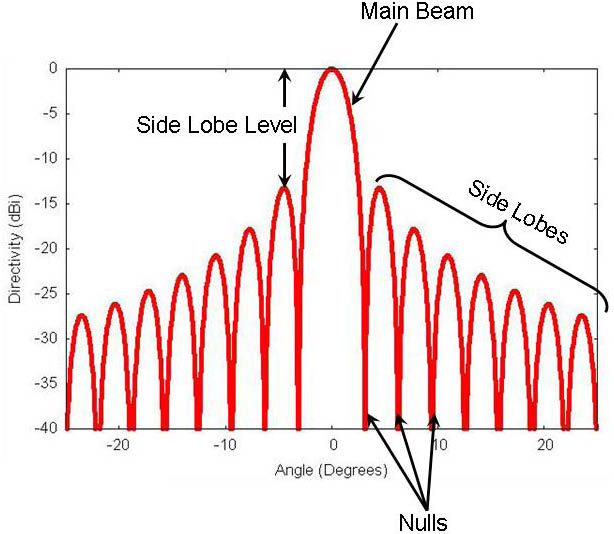
\includegraphics[height=0.7\textheight]{sinc.jpg}
    \caption*{\tiny{a rectangular aperture antenna radiation pattern}}
  \end{figure}
\end{frame}
% frame_
\begin{frame}
  \frametitle{}
  \begin{figure}
    
\includegraphics[height=0.8\textheight]{Thank_You.jpg}
%    \caption*{\tiny{kr=10000}}
  \end{figure}
\end{frame}


\end{document}
